%% ================================================================================================
%%  7. Simulation evidence
%%  Notes: research-agenda.md §7; details in C_simulation.tex
%%  Code: simulations/python/cultures.py, experiments.py (tables perf_*, manipulability, clones,
%%        theta_sweep), figures.py (fig_theta)
%% ================================================================================================
\section{Simulation evidence}\label{sec:simulation}

The propositions say what the procedure guarantees; they do not say how often the guarantees bite, nor
what they cost in the typical case. A Monte Carlo study answers both, and compares \QVC\ with twenty
other rules on the same elections.

\subsection{Design}

Each simulated election has 101 voters and 8 options: 7 open proposals and the status quo. The
proposals are made by voters drawn at random, near their own position, so that larger blocs propose more
and near-duplicates arise as they would under H1. Three electorates (``cultures'') are used:
\begin{itemize}
  \item \textbf{spatial}: voters' ideal points spread over a plane, preferences decreasing with distance;
  \item \textbf{polarised}: two blocs of 55\% and 45\% on either side of the plane, the case in which a
  compromise matters most;
  \item \textbf{impartial}: random independent rankings, a worst case for majority rule, reported in
  Appendix~\ref{app:simulation}.
\end{itemize}
Each voter vetoes the options beyond a personal tolerance, fixed before the proposals are known, so that
the veto reflects acceptability rather than the composition of the menu; on average a voter vetoes 35--40\% of
the options. Ballots are sincere, except in the manipulation study. Each rule is scored on:
\begin{itemize}
  \item \emph{Condorcet efficiency}: how often it elects the Condorcet winner when there is one;
  \item \emph{utility efficiency}: total utility of the winner, scaled from 0 for the average option to
  100 for the best \citep{Merrill1984};
  \item \emph{worst-off efficiency}: the same scale for the voter at the 10th percentile of utility, a
  measure of how well the least satisfied voters fare;
  \item \emph{acceptance}: the share of voters who do not veto the winner, and \emph{contested}: how often
  at least a third of the voters veto the winner;
  \item \emph{deadlock}: how often the status quo stays because nothing passes.
\end{itemize}
Details, calibration and the checks of the code are in Appendix~\ref{app:simulation}.

\subsection{Results}

% Generated by simulations/python/experiments.py -- do not edit by hand
\begin{table}[htbp]\centering\footnotesize
\setlength{\tabcolsep}{4pt}
\caption{The rules compared: polarised (55/45)}\label{tab:perf_polarised}
\sbox{\tabbox}{\begin{tabular}{l>{\raggedleft\arraybackslash}p{0.087\linewidth}>{\raggedleft\arraybackslash}p{0.087\linewidth}>{\raggedleft\arraybackslash}p{0.087\linewidth}>{\raggedleft\arraybackslash}p{0.087\linewidth}>{\raggedleft\arraybackslash}p{0.087\linewidth}>{\raggedleft\arraybackslash}p{0.087\linewidth}>{\raggedleft\arraybackslash}p{0.087\linewidth}}
\toprule
Rule & Condorcet eff. (\%) & Utility eff. (\%) & Worst-off eff. (\%) & Accepted (\%) & Contested (\%) & Deadlock (\%) & Fallback (\%) \\
\midrule
Plurality & 22.4 & 34.4 & 13.3 & 63.4 & 62.1 & 0.0 & 0.0 \\
IRV & 33.1 & 70.0 & 33.3 & 68.5 & 45.6 & 0.0 & 0.0 \\
Borda & 71.2 & 94.5 & 79.1 & 75.3 & 15.2 & 0.0 & 0.0 \\
Copeland & 100.0 & 97.2 & 85.3 & 76.7 & 9.8 & 0.0 & 0.0 \\
Minimax & 100.0 & 97.4 & 85.2 & 76.6 & 10.1 & 0.0 & 0.0 \\
Schulze & 100.0 & 97.4 & 85.2 & 76.6 & 10.1 & 0.0 & 0.0 \\
Ranked Pairs & 100.0 & 97.4 & 85.1 & 76.6 & 10.2 & 0.0 & 0.0 \\
Split Cycle & 100.0 & 97.4 & 85.2 & 76.6 & 10.1 & 0.0 & 0.0 \\
\midrule
Approval & 72.2 & 95.5 & 95.0 & 78.2 & 5.9 & 0.0 & 0.0 \\
Majority Judgment & 55.3 & 88.5 & 60.1 & 73.1 & 23.9 & 0.0 & 0.0 \\
\midrule
Fallback & 53.7 & 87.7 & 79.9 & 74.7 & 18.6 & 0.0 & 0.0 \\
Fallback (impasse) & 15.7 & 3.0 & 27.2 & 60.5 & 58.1 & 100.0 & 0.0 \\
Majoritarian compromise & 62.2 & 89.1 & 69.0 & 74.1 & 20.8 & 0.0 & 0.0 \\
Sequential veto & 38.7 & 74.1 & 64.4 & 71.6 & 30.7 & 0.0 & 0.0 \\
\midrule
Unanimity & 16.2 & 8.5 & 30.7 & 61.4 & 57.4 & 97.9 & 0.0 \\
PVC + Schulze & 90.8 & 96.2 & 86.7 & 76.6 & 10.2 & 0.0 & 0.0 \\
QVC, any veto (1/n) & 72.2 & 95.5 & 95.0 & 78.2 & 5.9 & 0.0 & 100.0 \\
QVC, 10\% & 72.4 & 95.6 & 95.0 & 78.2 & 5.9 & 0.0 & 98.6 \\
QVC, 25\% & 83.2 & 96.8 & 92.8 & 77.8 & 5.9 & 0.0 & 26.9 \\
QVC, 33\% & 94.3 & 97.7 & 88.4 & 77.1 & 5.9 & 0.0 & 5.9 \\
QVC, 50\% & 99.9 & 97.4 & 85.1 & 76.6 & 10.1 & 0.0 & 0.0 \\
\bottomrule
\end{tabular}}
\usebox{\tabbox}
\tabnotes{2,000 elections, 101 voters, 8 options of which one is the status quo. Condorcet efficiency: share of the elections with a Condorcet winner (here 97.7\%) in which the rule elects it. Utility efficiency: total utility of the winner, 0 for the average option and 100 for the best \citep{Merrill1984}. Worst-off efficiency: the same for the utility of the voter at the 10th percentile. Accepted: average share of the voters who do not veto the winner. Contested: share of the elections whose winner is vetoed by at least a third of the voters. Deadlock: the status quo stays because no proposal passes. Fallback: QVC excluded every option and kept the least vetoed. QVC, $x$: Condorcet with a blocking quota $\theta = x$ (Section~\ref{sec:procedure}). Monte Carlo standard errors are at most 1.1 points.}
{Monte Carlo simulation, cultures of \texttt{cultures.py}, rules of \texttt{voting.py}; \texttt{experiments.py}.}
\end{table}


\paragraph{Condorcet methods lead on welfare.} In both structured electorates, the Condorcet methods
(Copeland, Minimax, Schulze, Ranked Pairs, Split Cycle) reach the highest utility efficiency, 99.5 in
the spatial and 97.2--97.4 in the polarised electorate (Tables~\ref{tab:perf_polarised}
and~\ref{tab:perf_spatial}). Borda's rule and the evaluative rules (approval, Majority Judgment) come next;
plurality and instant-runoff trail far behind in the polarised case, where they elect a bloc's
favourite (utility efficiency 34 and 70). This confirms, with vetoes and an open agenda, the ranking of
\citet{Merrill1984} and \citet{GreenArmytageTidemanCosman2016}.

\paragraph{Hard vetoes deadlock.} Unanimity with the status quo as default keeps it in 98--99\% of
elections, and fallback bargaining with impasse never reaches an agreement: with 101 voters, no
proposal is acceptable to everyone. Their outcome is then the status quo, whose utility efficiency is close to that of a random option. This is Proposition~\ref{prop:gridlock} in numbers.

\paragraph{The veto quota buys protection for the worst-off.} In the polarised electorate, the Schulze
winner is vetoed by at least a third of the voters in 10.1\% of elections. \QVC(1/3) halves that, to
5.9\%, the minimum any rule can reach (Proposition~\ref{prop:acceptability}): in those 5.9\% of elections
every option is vetoed by a third. It raises worst-off efficiency from 85.2 to 88.4, and it does so with
no loss of total utility (97.7 against 97.4): the compromise it picks is better for the minority bloc
and about as good on average. The cost is in Condorcet efficiency, 94.3\%: in 5.7\% of the elections that have a Condorcet winner, the
majority's preferred option is set aside because a blocking third rejects it. With $\theta = 1/4$ the
trade goes further (worst-off efficiency 92.8, Condorcet efficiency 83.2), towards the ``least-vetoed''
outcome of approval voting. In the spatial electorate, where most options are broadly acceptable,
\QVC(1/3) and Schulze agree in 99.5\% of cases with a Condorcet winner. The proportional veto core with
Schulze moves in the same direction as \QVC\ but less (worst-off efficiency 86.7, contested 10.2\%).

% Generated by simulations/python/experiments.py -- do not edit by hand
\begin{table}[htbp]\centering\footnotesize
\setlength{\tabcolsep}{4pt}
\caption{The rules compared: spatial (2D)}\label{tab:perf_spatial}
\sbox{\tabbox}{\begin{tabular}{l>{\raggedleft\arraybackslash}p{0.087\linewidth}>{\raggedleft\arraybackslash}p{0.087\linewidth}>{\raggedleft\arraybackslash}p{0.087\linewidth}>{\raggedleft\arraybackslash}p{0.087\linewidth}>{\raggedleft\arraybackslash}p{0.087\linewidth}>{\raggedleft\arraybackslash}p{0.087\linewidth}>{\raggedleft\arraybackslash}p{0.087\linewidth}}
\toprule
Rule & Condorcet eff. (\%) & Utility eff. (\%) & Worst-off eff. (\%) & Accepted (\%) & Contested (\%) & Deadlock (\%) & Fallback (\%) \\
\midrule
Plurality & 41.5 & 73.1 & 67.0 & 76.7 & 11.7 & 0.0 & 0.0 \\
IRV & 64.9 & 92.0 & 86.3 & 80.0 & 1.9 & 0.0 & 0.0 \\
Borda & 86.3 & 98.6 & 93.8 & 81.1 & 1.3 & 0.0 & 0.0 \\
Copeland & 100.0 & 99.5 & 94.9 & 81.3 & 1.1 & 0.0 & 0.0 \\
Minimax & 100.0 & 99.5 & 95.0 & 81.3 & 1.1 & 0.0 & 0.0 \\
Schulze & 100.0 & 99.5 & 95.0 & 81.3 & 1.1 & 0.0 & 0.0 \\
Ranked Pairs & 100.0 & 99.5 & 94.9 & 81.2 & 1.1 & 0.0 & 0.0 \\
Split Cycle & 100.0 & 99.5 & 95.0 & 81.3 & 1.1 & 0.0 & 0.0 \\
\midrule
Approval & 78.2 & 97.6 & 94.8 & 81.8 & 0.9 & 0.0 & 0.0 \\
Majority Judgment & 77.7 & 97.6 & 91.6 & 80.8 & 1.1 & 0.0 & 0.0 \\
\midrule
Fallback & 61.2 & 90.4 & 86.5 & 79.7 & 4.2 & 0.0 & 0.0 \\
Fallback (impasse) & 12.1 & -2.0 & -0.6 & 61.8 & 50.8 & 100.0 & 0.0 \\
Majoritarian compromise & 76.6 & 97.1 & 92.0 & 80.8 & 1.6 & 0.0 & 0.0 \\
Sequential veto & 45.2 & 81.8 & 76.9 & 78.0 & 8.4 & 0.0 & 0.0 \\
\midrule
Unanimity & 12.1 & -0.9 & 0.3 & 62.1 & 50.6 & 99.4 & 0.0 \\
PVC + Schulze & 99.5 & 99.5 & 94.8 & 81.3 & 1.1 & 0.0 & 0.0 \\
QVC, any veto (1/n) & 78.2 & 97.6 & 94.8 & 81.8 & 0.9 & 0.0 & 100.0 \\
QVC, 10\% & 78.3 & 97.6 & 94.8 & 81.8 & 0.9 & 0.0 & 96.9 \\
QVC, 25\% & 96.1 & 99.2 & 94.9 & 81.4 & 0.9 & 0.0 & 9.2 \\
QVC, 33\% & 99.5 & 99.5 & 94.9 & 81.3 & 0.9 & 0.0 & 0.9 \\
QVC, 50\% & 100.0 & 99.5 & 95.0 & 81.3 & 1.1 & 0.0 & 0.0 \\
\bottomrule
\end{tabular}}
\usebox{\tabbox}
\tabnotes{2,000 elections, 101 voters, 8 options of which one is the status quo. Condorcet efficiency: share of the elections with a Condorcet winner (here 98.6\%) in which the rule elects it. Utility efficiency: total utility of the winner, 0 for the average option and 100 for the best \citep{Merrill1984}. Worst-off efficiency: the same for the utility of the voter at the 10th percentile. Accepted: average share of the voters who do not veto the winner. Contested: share of the elections whose winner is vetoed by at least a third of the voters. Deadlock: the status quo stays because no proposal passes. Fallback: QVC excluded every option and kept the least vetoed. QVC, $x$: Condorcet with a blocking quota $\theta = x$ (Section~\ref{sec:procedure}). Monte Carlo standard errors are at most 1.1 points.}
{Monte Carlo simulation, cultures of \texttt{cultures.py}, rules of \texttt{voting.py}; \texttt{experiments.py}.}
\end{table}


\paragraph{Only clone-independent rules resist flooding.} Adding three clones of a losing option never
changes the outcome of Schulze, Ranked Pairs, Split Cycle or \QVC\ (Table~\ref{tab:clones}). It changes
that of Borda's rule in 14--24\% of elections (teaming), of fallback bargaining in 25--36\%, of the
majoritarian compromise in 23--52\%, of sequential vetoes in 68--82\%, and of the proportional veto core
in up to 54\%. Cloning the winner defeats it under plurality in 94--100\% of elections (vote splitting).

% Generated by simulations/python/experiments.py -- do not edit by hand
\begin{table}[htbp]\centering\footnotesize
\setlength{\tabcolsep}{4pt}
\caption{Share of outcomes changed by three clones}\label{tab:clones}
\sbox{\tabbox}{\begin{tabular}{l>{\raggedleft\arraybackslash}p{0.098\linewidth}>{\raggedleft\arraybackslash}p{0.100\linewidth}>{\raggedleft\arraybackslash}p{0.100\linewidth}>{\raggedleft\arraybackslash}p{0.100\linewidth}>{\raggedleft\arraybackslash}p{0.100\linewidth}>{\raggedleft\arraybackslash}p{0.100\linewidth}}
\toprule
Rule & Spatial: loser (\%) & Spatial: winner (\%) & Polarised: loser (\%) & Polarised: winner (\%) & Impartial: loser (\%) & Impartial: winner (\%) \\
\midrule
Plurality & 0.0 & 97.6 & 0.0 & 93.7 & 0.0 & 100.0 \\
IRV & 0.3 & 0.2 & 0.2 & 0.3 & 1.2 & 1.9 \\
Borda & 14.1 & 1.2 & 24.3 & 3.1 & 21.4 & 1.4 \\
Copeland & 0.2 & 0.3 & 0.5 & 0.3 & 7.7 & 3.0 \\
Minimax & 0.0 & 1.2 & 0.0 & 1.9 & 0.0 & 2.0 \\
Schulze & 0.0 & 0.0 & 0.0 & 0.0 & 0.0 & 0.0 \\
Ranked Pairs & 0.0 & 0.0 & 0.0 & 0.0 & 0.0 & 0.0 \\
Split Cycle & 0.0 & 0.0 & 0.0 & 0.0 & 0.0 & 0.0 \\
\midrule
Approval & 0.0 & 0.0 & 0.0 & 0.0 & 0.0 & 0.2 \\
Majority Judgment & 0.0 & 0.0 & 0.0 & 0.0 & 0.0 & 0.0 \\
\midrule
Fallback & 30.7 & 0.0 & 36.4 & 0.0 & 24.6 & 0.0 \\
Fallback (impasse) & 0.0 & 0.0 & 0.0 & 0.0 & 0.0 & 0.0 \\
Majoritarian compromise & 23.1 & 12.8 & 34.1 & 28.2 & 51.9 & 14.9 \\
Sequential veto & 67.8 & 0.0 & 68.7 & 0.0 & 81.9 & 0.0 \\
\midrule
Unanimity & 0.0 & 0.0 & 0.0 & 0.0 & 0.0 & 0.0 \\
PVC + Schulze & 1.2 & 0.0 & 15.1 & 0.1 & 53.9 & 4.5 \\
QVC, any veto (1/n) & 0.0 & 0.0 & 0.0 & 0.0 & 0.0 & 0.0 \\
QVC, 10\% & 0.0 & 0.0 & 0.0 & 0.0 & 0.0 & 0.0 \\
QVC, 25\% & 0.0 & 0.0 & 0.0 & 0.0 & 0.0 & 0.0 \\
QVC, 33\% & 0.0 & 0.0 & 0.0 & 0.0 & 0.0 & 0.0 \\
QVC, 50\% & 0.0 & 0.0 & 0.0 & 0.0 & 0.0 & 0.0 \\
\bottomrule
\end{tabular}}
\usebox{\tabbox}
\tabnotes{1,000 elections per culture, 101 voters, 8 options. Loser: three clones of a losing option, drawn at random, are added (teaming, or flooding the agenda); winner: three clones of the winner are added (vote splitting). A clone is a variant that every voter ranks next to the original, and grades and vetoes as the original \citep{Tideman1987}. The outcome is unchanged if the winner is the same or a clone of it. Monte Carlo standard errors at most 1.6 points.}
{Monte Carlo simulation, cultures of \texttt{cultures.py}, rules of \texttt{voting.py}; \texttt{experiments.py}.}
\end{table}


\paragraph{Vetoes are a strategic instrument.} Table~\ref{tab:manipulability} reports how often a
coalition of voters who prefer some option $y$ to the winner can elect $y$ with simple joint strategies:
ranking $y$ first and the winner last, and vetoing the winner or every option but $y$. With full coalitions, most decisive rules are manipulable in a majority of elections, as the
Gibbard--Satterthwaite theorem leads one to expect (instant-runoff is the least exposed, as in
\citealp{GreenArmytageTidemanCosman2016}); \QVC\ with $\theta < 1/2$ in nearly all, because the voters who prefer $y$ to the
winner usually number more than $\theta n$ and can veto the winner (Proposition~\ref{prop:blocking}).
The more realistic case is a small coalition, at most 10\% of the voters. Schulze, Ranked Pairs, Split Cycle and Minimax are then manipulable in only 4--7\% of structured
elections (Copeland in 20--31\%), against 37--45\% for instant-runoff and 69--85\% for
approval voting and Majority Judgment. \QVC(1/3) stands between, at 11\% in the spatial and 27\% in the
polarised electorate; \QVC(1/4) at 52--57\%. Under the impartial culture all rules are highly
manipulable. Unanimity is almost never manipulable, for the wrong reason: it rarely decides anything.

% Generated by simulations/python/experiments.py -- do not edit by hand
\begin{table}[htbp]\centering\footnotesize
\setlength{\tabcolsep}{4pt}
\caption{Share of elections a coalition can manipulate}\label{tab:manipulability}
\sbox{\tabbox}{\begin{tabular}{l>{\raggedleft\arraybackslash}p{0.089\linewidth}>{\raggedleft\arraybackslash}p{0.089\linewidth}>{\raggedleft\arraybackslash}p{0.100\linewidth}>{\raggedleft\arraybackslash}p{0.100\linewidth}>{\raggedleft\arraybackslash}p{0.100\linewidth}>{\raggedleft\arraybackslash}p{0.100\linewidth}}
\toprule
Rule & Spatial: all (\%) & Spatial: 10\% (\%) & Polarised: all (\%) & Polarised: 10\% (\%) & Impartial: all (\%) & Impartial: 10\% (\%) \\
\midrule
Plurality & 94.2 & 53.8 & 98.6 & 45.0 & 100.0 & 98.0 \\
IRV & 47.8 & 36.6 & 76.2 & 44.6 & 53.4 & 51.6 \\
Borda & 97.8 & 79.0 & 96.8 & 81.6 & 100.0 & 95.2 \\
Copeland & 96.2 & 19.8 & 96.8 & 31.2 & 100.0 & 88.4 \\
Minimax & 63.2 & 4.8 & 53.8 & 7.0 & 100.0 & 70.8 \\
Schulze & 63.2 & 4.8 & 53.8 & 6.8 & 100.0 & 71.2 \\
Ranked Pairs & 71.6 & 4.4 & 69.8 & 6.2 & 100.0 & 64.8 \\
Split Cycle & 73.0 & 5.0 & 72.2 & 7.2 & 100.0 & 72.2 \\
\midrule
Approval & 99.6 & 84.6 & 100.0 & 68.8 & 100.0 & 90.6 \\
Majority Judgment & 98.8 & 79.0 & 99.4 & 79.8 & 100.0 & 86.6 \\
\midrule
Fallback & 83.6 & 97.4 & 86.2 & 98.8 & 100.0 & 90.6 \\
Fallback (impasse) & 5.8 & 0.0 & 15.8 & 0.0 & 0.0 & 0.0 \\
Majoritarian compromise & 77.2 & 33.0 & 81.2 & 39.4 & 100.0 & 81.6 \\
Sequential veto & 76.8 & 76.8 & 63.2 & 63.2 & 69.2 & 69.2 \\
\midrule
Unanimity & 0.0 & 0.0 & 0.8 & 0.8 & 0.0 & 0.0 \\
PVC + Schulze & 98.4 & 5.8 & 87.6 & 7.0 & 100.0 & 95.4 \\
QVC, any veto (1/n) & 99.6 & 84.6 & 100.0 & 68.8 & 100.0 & 90.6 \\
QVC, 10\% & 99.6 & 84.6 & 100.0 & 68.8 & 100.0 & 90.6 \\
QVC, 25\% & 99.6 & 51.8 & 100.0 & 56.8 & 100.0 & 90.6 \\
QVC, 33\% & 99.4 & 11.0 & 100.0 & 26.6 & 100.0 & 81.8 \\
QVC, 50\% & 72.2 & 4.8 & 83.6 & 7.0 & 100.0 & 71.2 \\
\bottomrule
\end{tabular}}
\usebox{\tabbox}
\tabnotes{500 elections per culture, 101 voters, 8 options. An election counts as manipulable if, for some option $y$, voters who prefer $y$ to the winner can elect $y$ by one of three joint strategies: rank $y$ first and the winner last, vetoing the winner; the same, vetoing every option but $y$; or rank the winner last and veto it. All: every voter who prefers $y$ to the winner joins; 10\%: at most 10 of them. Other strategies may succeed where these fail: the shares are lower bounds. Monte Carlo standard errors at most 2.2 points.}
{Monte Carlo simulation, cultures of \texttt{cultures.py}, rules of \texttt{voting.py}; \texttt{experiments.py}.}
\end{table}


\paragraph{The trade-off in the quota.} Figure~\ref{fig:theta} traces the measures as $\theta$ varies.
Condorcet efficiency rises and worst-off efficiency falls with $\theta$; the fallback, frequent below
20\%, all but disappears above 30\%; small-coalition manipulability falls steeply between 20\% and 40\%.
At $\theta = 1/3$ the fallback is rare (1\% of spatial and 6\% of polarised elections), Condorcet
efficiency is at least 94\% and most of the gain in worst-off efficiency is kept; a quarter buys more protection at the price of a fallback in a quarter of polarised elections and two
to four times the small-coalition manipulability.

\begin{figure}[htbp]\centering
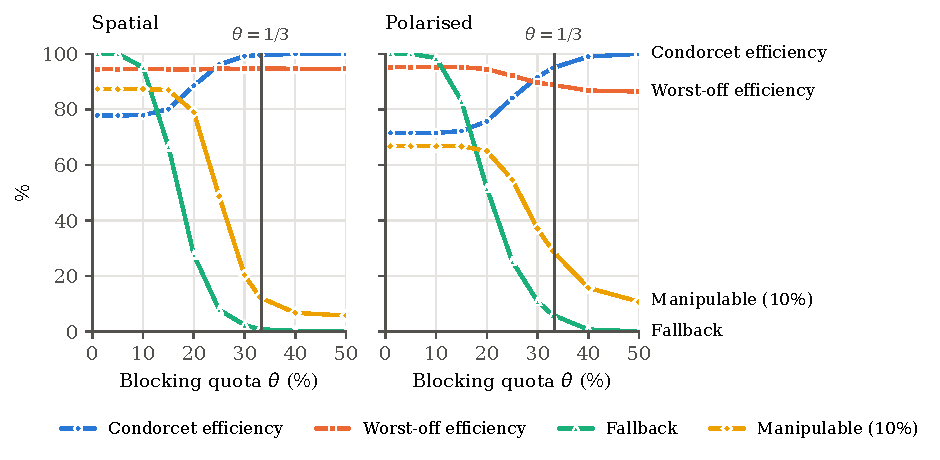
\includegraphics[width=\linewidth]{fig_theta}
\caption{QVC: what the blocking quota buys and costs}\label{fig:theta}
\figurenotes{Each line is a measure of the winner of \QVC($\theta$) as the blocking quota $\theta$
varies, from a single veto ($1/n$, plotted at 1\%) to half of the voters. Condorcet efficiency,
worst-off efficiency and fallback as in Table~\ref{tab:perf_polarised}; manipulable (10\%): share of
elections a coalition of at most 10\% of the voters can manipulate (Table~\ref{tab:manipulability}).
1,000 elections per culture (300 for manipulability), 101 voters, 8 options. The vertical line marks the
recommended quota, $\theta = 1/3$. Values in Table~\ref{tab:theta_sweep}.}{Monte Carlo simulation,
\texttt{experiments.py}; \texttt{figures.py}.}
\end{figure}

\subsection{What the simulation does not show}

The cultures are stylised: two dimensions, Euclidean preferences, a fixed tolerance for vetoes, and a
proposal process with no deliberation. The manipulation study gives full information to the coalition
and only counts three strategies, so it bounds manipulability from below; it does not model the
safeguards of Section~\ref{sec:safeguards}, which act on the willingness to veto strategically rather
than on the counting rule. Ballots from real assemblies, for instance from the PrefLib library
\citep{MatteiWalsh2013}, would test the conclusions on observed preferences; Debian's published ballots
would be a natural start.
